% This must be in the first 5 lines to tell arXiv to use pdfLaTeX, which is strongly recommended.
\pdfoutput=1
% In particular, the hyperref package requires pdfLaTeX in order to break URLs across lines.

\documentclass[11pt]{article}

% Remove the "review" option to generate the final version.
\usepackage[]{ACL2023}

% Standard package includes
\usepackage{times}
\usepackage{latexsym}

% For proper rendering and hyphenation of words containing Latin characters (including in bib files)
\usepackage[T1]{fontenc}
% For Vietnamese characters
% \usepackage[T5]{fontenc}
% See https://www.latex-project.org/help/documentation/encguide.pdf for other character sets

% This assumes your files are encoded as UTF8
\usepackage[utf8]{inputenc}

% This is not strictly necessary, and may be commented out.
% However, it will improve the layout of the manuscript,
% and will typically save some space.
\usepackage{microtype}

% This is also not strictly necessary, and may be commented out.
% However, it will improve the aesthetics of text in
% the typewriter font.
\usepackage{inconsolata}

% Other
% \usepackage{hyperref}
\usepackage{graphicx}

% If the title and author information does not fit in the area allocated, uncomment the following
%
%\setlength\titlebox{<dim>}
%
% and set <dim> to something 5cm or larger.

\title{Data Augmentation for Natural Language Inference}

% Author information can be set in various styles:
% For several authors from the same institution:
% \author{Author 1 \and ... \and Author n \\
%         Address line \\ ... \\ Address line}
% if the names do not fit well on one line use
%         Author 1 \\ {\bf Author 2} \\ ... \\ {\bf Author n} \\
% For authors from different institutions:
% \author{Author 1 \\ Address line \\  ... \\ Address line
%         \And  ... \And
%         Author n \\ Address line \\ ... \\ Address line}
% To start a seperate ``row'' of authors use \AND, as in
% \author{Author 1 \\ Address line \\  ... \\ Address line
%         \AND
%         Author 2 \\ Address line \\ ... \\ Address line \And
%         Author 3 \\ Address line \\ ... \\ Address line}

\author{Tianyuan Qiu \\
  520030910137 \\
  \texttt{frank\_qiu@sjtu.edu.cn} \\}

\begin{document}
\maketitle
\begin{abstract}
This paper proposes enhancing the performance of the BERT base model for Natural Language Inference (NLI) through data augmentation techniques. The study focuses on generating additional training samples by modifying the original dataset using strategies like synonym and antonym substitution. Experiments on a benchmark NLI dataset demonstrate that data augmentation significantly improves the accuracy of the BERT base model. The findings highlight the potential of data augmentation in enhancing NLI models and contribute to research on NLP and data augmentation. The problems reflected in the results are also discuessed and directions for further improvement are proposed. Code related to the study is publicly available at \url{https://github.com/PaperL/Toy_NLI}
\end{abstract}

\section{Introduction}

\subsection{Natural Language Inference}

The semantic concepts of entailment and contradiction are central to all aspects of natural language meaning, from the lexicon to the content of entire texts. Natural Language Inference (NLI) is a task that aims to determine the logical relationship between two given sentences, which can be categorized as entailment, contradiction, or neutrality. This task is of significant importance in various natural language processing applications, including question answering, summarization, and sentiment analysis. To successfully perform NLI, a comprehensive understanding of semantic and syntactic structures is necessary in order to make accurate inferences about the relationship between the provided sentences.\cite{bowman2015large}

\subsection{Data Augmentation}

Data augmentation is a technique used to expand the training dataset by generating additional samples through various modifications or transformations applied to the original data. \cite{feng2021survey} In the context of NLI, data augmentation can involve techniques such as synonym substitution, paraphrasing, or back-translation. By introducing diverse examples, data augmentation aims to enhance the model's generalization ability, improve robustness, and mitigate overfitting, ultimately boosting the performance of NLI models.

\subsection{BERT Model}

The BERT (Bidirectional Encoder Representations from Transformers) model is a state-of-the-art pre-trained language model that utilizes Transformer architecture to capture contextual information from text.\cite{devlin2018bert} BERT has achieved remarkable success in various NLP tasks due to its ability to learn bidirectional representations of words. It has been widely adopted as a baseline model for many NLP applications, including the NLI task.

% \footnote{\url{https://2023.aclweb.org/calls/main_conference/}}\texttt{anthology.bib}

\section{Data Augmentation for NLP Task}

Data plays a crucial role in achieving high performance in machine learning models, and the more data we have, the better results we can obtain. However, manually annotating a large amount of training data can be a luxury in terms of time and resources. To overcome this challenge, data augmentation techniques come into play, offering a way to enhance model performance by generating synthetic training data. While data augmentation is widely popular in the field of computer vision, applying it to natural language processing (NLP) tasks poses unique challenges due to the complexity of language.\\

In computer vision, augmenting images is relatively straightforward. Techniques such as flipping, adding noise, or cropping can be easily applied using libraries like imgaug, leading to improved performance in vision models. Augmentation has been proven to be a key factor in the success of computer vision models.\\

However, augmenting text in NLP is more intricate. Not every word can be easily replaced with alternatives like "a," "an," or "the," and not every word has a direct synonym. Moreover, even a slight change in a word can drastically alter the context and meaning of a sentence. Unlike images, where introducing noise or cropping may still allow the model to classify the image correctly, the same level of simplicity does not apply to text augmentation.\\

Given the limitation of manually creating an unlimited amount of training data, researchers have explored various methods to generate more data for model training.\\

\subsection{Thesaurus}
Zhang et al. found that one of the useful ways to do text augmentation is by replacing words or phrases with their synonyms.\cite{NIPS2015_250cf8b5} Leveraging existing thesaurus help to generate lots of data in a short time. Zhang et al. select a word and replace it with synonyms according to the geometric distribution.\\

\subsection{Word Embeddings}
Wang and Yang introduced a data augmentation approach for automatic categorization of annoying behaviors.\cite{wang2015s} They proposed two methods for finding similar words for replacement. The first method involved utilizing k-nearest-neighbor (KNN) and cosine similarity to identify similar words. As an alternative, they also explored the use of pre-trained classic word embeddings such as word2vec, GloVe, and fasttext to perform similarity searches. These techniques aimed to enhance the data augmentation process and improve the accuracy of the automatic categorization model.\\

\subsection{Back Translation}
In the field of machine translation, back-translation has been employed as a data augmentation technique to address the issue of limited training data for certain language pairs. Sennrich et al. utilized back-translation to augment the training data for low-resource translation models.\cite{sennrich2015improving} By translating the target language sentences back to the source language and combining them with the original source sentences, the number of training examples from the source language to the target language could be significantly increased, thereby improving the performance of the translation model.

\subsection{Contextualized Word Embeddings}
Fadaee et al. introduced the use of contextualized word embeddings as a form of text augmentation in the context of low-resource neural machine translation.\cite{fadaee2017data} Instead of relying on static word embeddings, they leveraged contextualized word embeddings to replace target words in the translation process. This approach, known as Translation Data Augmentation (TDA), demonstrated improvements in the machine translation model's performance by leveraging the power of contextualized embeddings and is further confirmed in other work.\cite{kobayashi2018contextual}

\subsection{Text Generation}
Kafle et al. proposed an alternative approach to text augmentation for visual question answering by generating augmented data through text generation techniques.\cite{kafle2017data} They presented two approaches: template augmentation and LSTM-based question generation. Template augmentation involved using pre-defined question templates that could be paired with rule-based answers, while the LSTM-based approach utilized image features to generate questions. By generating complete sentences instead of replacing individual words, Kafle et al. aimed to enhance the diversity and quality of the augmented data, contributing to improved performance in visual question answering tasks.


\section{Experiment}

The experimental environment is \textit{WSL2 (Ubuntu 20.04) under Windows 10}, using \textit{python3} and \textit{pyTorch}. Specific code and package requirements is attached.

\subsection{Data Preprocessing}

In summary, the data preprocessing pipeline reads the input data, extracts relevant tokens, augments the texts by replacing adjectives and verbs with synonyms and antonyms, generates new augmented examples. Then determine the proper token length according to the dataset. And finally saves the preprocessed data for follow-up use in text classification tasks using deep learning models.

\subsubsection{Word Augmentation}
The objective of preprocessing is to augment the existing data by replacing adjectives and verbs in the input texts and generate new data samples for improved training.

First, data are read from a JSONL file and the \texttt{spacy} library is utilized to extract adjectives and verbs from a given sentence.\footnote{\url{https://spacy.io/}} These extracted adjectives and verbs serve as the targets for augmentation. To modify these words while preserving the correctness of the example, the \texttt{nlpaug} library is employed.\footnote{\url{https://github.com/makcedward/nlpaug}} The augmenters in \texttt{nlpaug} are based on the \texttt{nltk} toolchain. The tense is maintained using the \texttt{en\_core\_web\_sm} model provided by \texttt{spacy}. The tense of words is indicated by the tags generated by the \texttt{spacy} model, and any undesirable augmented data is discarded.

The \texttt{SynonymAug} augmenter replaces words with similar meanings while keeping the label unchanged. On the other hand, the \texttt{AntonymAug} augmenter replaces words with opposite meanings. Several situations can arise: if the label of the example is \textit{neutral}, reversing word meanings does not have a significant impact; if the label is \textit{entailment}, reversing word meanings should result in a contradiction; if the label is \textit{contradiction}, reversing a random number of words introduces uncertainty to the label, as the reversal may lead to either less conflict (entailment), more conflict (contradiction), or a broken relationship (neutral).

After the replacement process, the program checks if the augmented texts are different from the originals and constructs new examples accordingly, because augmenter sometimes returns the same words. If a synonym-replaced text is different, it creates an augmented example and appends it to the augmented data list. Antonym-replaced text is checked similarly. In addition, the program utilizes parallel processing with a \texttt{Pool} to efficiently process the data examples in parallel.

\subsubsection{Tokenization}

Tokenization is a fundamental process that involves splitting a sequence of text into individual tokens or words. In our study, we analyzed and determined the length of tokens in the given dataset to facilitate the tokenization process.

To ensure compatibility with the PyTorch model's input data requirement of having the same length, we needed to establish a maximum token length. This decision was based on an analysis of the distribution of sequence lengths within our dataset. We employed the \texttt{AutoTokenizer} from the \texttt{transformers} library to examine the token lengths of the text pairs. By calculating the sequence lengths for each text pair, we determined the maximum token length that would encompass a greater number of examples, particularly those with shorter lengths, thereby reducing computational complexity.

For the tokenization process, we utilized the \texttt{BertTokenizer} provided by the \texttt{transformers} library. This tokenizer converts the input text into a suitable format for the BERT model. We performed preprocessing on both the training and test datasets using the \texttt{preprocess\_dataset} function. The sequences were padded to the maximum token length, and the resulting tokenized inputs included the \texttt{input\_ids}, \texttt{attention\_mask}, and \texttt{token\_type\_ids}.

To conform to the data format required by the deep learning model, we quantized the label information. In this quantization scheme, the label "0" represents \textit{entailment}, "1" represents \textit{contradiction}, and "2" represents \textit{neutral}. Prior research has demonstrated the effectiveness of this quantification approach, and the order of the labels does not impact the results \cite{chen2015convolutional}.

Practically, tokenization results in a data size increase of less than 10 times. Since the text data itself occupies relatively less space, preprocessing the data beforehand rather than during model execution can significantly improve training efficiency.


\subsection{Model Training}

Experimental Platform: \textit{Ubuntu 20.04, Cuda 11.3, PyTorch 1.11.0, Python 3.8}. Experimental device: one \textit{A100-PCIE-40GB}. Each epoch performs training using all the data. Batch size is set to 32, and the \textit{AdamW} optimizer is used with a learning rate of 2e-5. The loss function used is \textit{CrossEntropyLoss}. No additional components were added except for Bert Base uncased.

\section{Result and Review}

\subsection{Dataset Preprocessing}

\begin{figure*}[t]
  \centering
  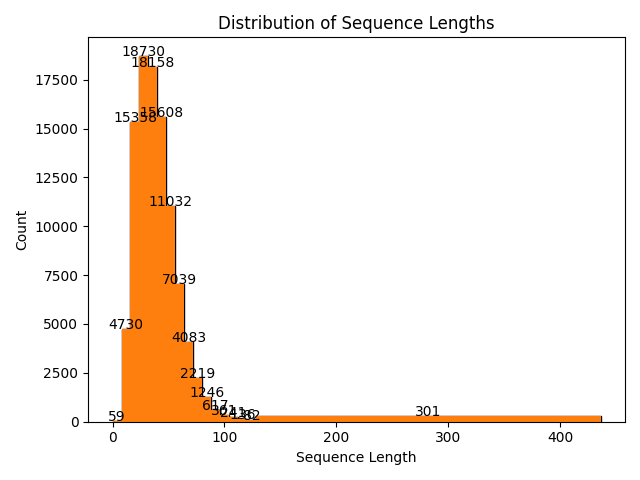
\includegraphics[width=0.6\textwidth]{distribution.png}
  \caption{Distribution of sequence lengths of given dataset using tokenizer from Bert.}
  \label{fig:image_label}
\end{figure*}

As shown in the above figure, texts longer than 128 tokens account for less than 0.3\% of all texts. Therefore, during the tokenization process, the max length is set to 128, and any text exceeding this limit is truncated. The loss of these truncated contents does not have a perceptible negative impact on the training results.

In addition, a total of 92,567 new samples were generated, effectively doubling the available dataset. Here are some examples (original text and augmented text):

\begin{verbatim}
SYNONYM:
i think we might exist capable to assist.
i think we might be able to help.
SYNONYM:
a launch to say let's preserve to a greater
extent because he never said that
a launch to say let's conserve more because
he never said that
ANTONYM:
well it's been very nasty talking to you
well it's been very nice talking to you
ANTONYM:
i think we might be unable to help.
i think we might be able to help.
\end{verbatim}


\section{Model Evaluation}

The author conducted experiments using the unenhanced dataset and the Bert Base uncased model as the baseline. Compare the training process with an augmented dataset to observe and analyze the impact of data augmentation on the Natural Language Inference task.

In both the baseline and data augmentation experiments, the initial loss was above 0.8 and eventually converged to around 0.6. The training with the augmented dataset showed significantly better results compared to the original dataset. The comparison was based on the decrease in loss for the same batch size. After training on 1 million samples (approximately 10 epochs for the baseline and 5 epochs for data augmentation), the augmented model approached convergence with a loss below 0.65, while the baseline model remained around 0.7.

Furthermore, when training on 3 million samples (approximately 30 epochs for the baseline and 15 epochs for data augmentation), both models achieved relatively stable losses. Evaluation using a test dataset showed an improvement of approximately 0.6\% in accuracy for the data augmentation approach.

\section{Review}

This study demonstrates the positive impact of data augmentation on improving model performance by comparing the training of the same pretrained model on augmented and original datasets for NLI tasks. However, the evaluation of model performance and the results of manually curated datasets suggest that the effectiveness of data augmentation in the NLP field still needs improvement when using non-massive models such as GPT-3. In this work, multiple commonly used NLP tools were employed, revealing two common deficiencies. Firstly, during the process of word replacement, particularly with verbs, it is challenging for the processing algorithm to ensure the preservation of tense and voice in the replacement results. This may be attributed to the lack of harmonious analysis at the sentence level in the replacement program. Secondly, in terms of changes involving synonyms and antonyms, the use of deep learning models results in a high error rate. This might be due to the inability of deep learning tasks' datasets to accurately reflect the lexical meanings of words, leading to a higher number of errors during word-level replacement. To address this issue, it may be necessary to strengthen the application of traditional algorithms that focus on dictionary processing.

\section*{Acknowledgements}
This is the Course Project of the 2023 NLU Course taught by Professor Hai Zhao, with Yao Yao serving as the teaching assistant. I would like to express our sincere gratitude to Professor Zhao for his incredibly insightful lectures and to the teaching assistant for assigning excellent assignments and providing meticulous feedback. I also extend our thanks to our classmates for their valuable discussions.

% Entries for the entire Anthology, followed by custom entries
\bibliography{custom}
\bibliographystyle{acl_natbib}


\appendix

\section{Appendix}
\label{sec:appendix}

Content of \url{https://github.com/PaperL/Toy_NLI} is attached.

\end{document}
